\section{Introduction}
\label{sec:introduction}

Since its appearance in late 2017, the total USD value locked (TVL) in decentralized finance (DeFi) protocols has seen an exponential growth\cite{how-to-defi-advanced} giving it the potential to rise to one of the most important cornerstones in the crypto world in the upcoming years (see Fig.\,\ref{fig:tvl}).
\begin{figure}
    \centering
    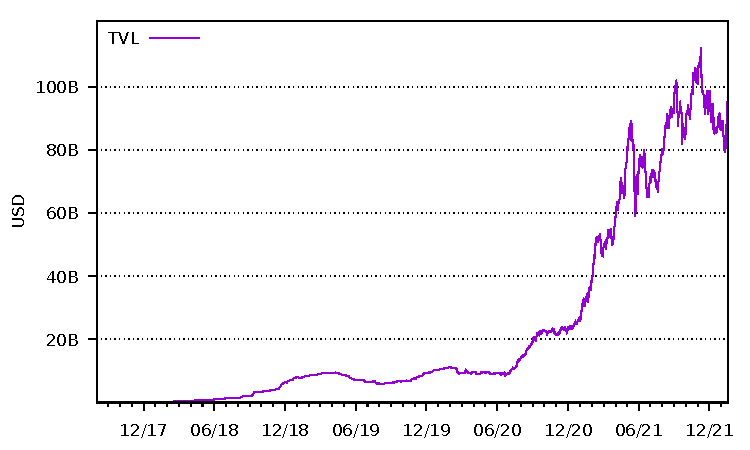
\includegraphics[width=\textwidth]{figures/tvl.pdf}
    \vskip1em
    \caption{The development of the total USD value locked in DeFi protocols since August 2017 (08/17) - data obtained from \textit{DeFi Pulse}.\cite{defi-pulse}}
    \label{fig:tvl}
\end{figure}
The high returns that can be achieved within the DeFi ecosystem attract institutional capital in addition to traditional investors.\cite{defi-report-q2-2021}
Today, the boundaries of financial theories are being tested daily, and more and more decentralized applications are joining the ecosystem.
This growing number of participants is accelerating the progression of concepts such as liquidity pools,\cite{schar2021} flash loans,\cite{wang2021} yield farming,\cite{cousaert2021} and stablecoins.\cite{zhao2021}
The latter are important components in DeFi as they enable investors to generate yield on their crypto assets while alleviating the potential adverse effect of market volatility.\cite{kristoufek2020}
Despite the steady increase in demand for stablecoins (six-fold growth in between 10/20 and 10/21),\cite{stablecoin-report} lending rates remain high,\cite{aave} indicating that demand is in excess.\\[-1em]

Stablecoins can be classified into three major classes: First generation stablecoins are off-chain and supposed to be backed-up by bank deposits and regular auditing (\textit{e.g.}, \textsc{USDC},\cite{usdc} \textsc{Tether}\cite{tether}, and \textsc{wbtc}\cite{wbtc}).\cite{griffin2020}
Second generation stablecoins are on-chain, associated with cryptocurrency collaterals, and thus embedding high-quality collaterals in a traceable sense (\textsc{DAI}\cite{dai}).\cite{fatas2019}
Third generation stablecoins are algorithm-based and function through a combination of endogenous and exogenous collateral ranging from totally endogenous (\textit{e.g.}, \textsc{UST}\cite{ust}) to partially collateralised (\textit{e.g.}, \frax\cite{frax}).\\[-1em]

The rules that define how algorithmic stablecoins work are defined in smart contracts that can only change by leveraging social consensus or \textit{via} governance votes.
Typical smart contract functions enable, \textit{e.g.}, the minting and burning of tokens or the communication to services outside the blockchain through oracles.\cite{breidenbach2021}
Overall, the primary logic underpinning the functions of algorithm-based stablecoins relies on tokens being burned or minted when the price of the stable fluctuates from the predefined stable value - commonly referred to as its peg. Thus the algorithm would facilitate the minting of new tokens for cases where the price of the stablecoin falls below the peg, and would burn new tokens in cases where the price is over the peg. This mechanism is referred as maintaining the peg.
The price stability of a stablecoin is strongly correlated to the project-owned liquidity. 
If there is only limited liquidity available, then it is easy to manipulate the market value of such an asset, which results in an unbalanced peg.
The consequences can range from severe financial damages for investors to bankruptcy of the project.\\

Our goal is the creation of a suite of tools that enables the enforcement of stablecoin pegs by levering cashflow generating assets and fees from protocol-owned liquidity to funnel stability towards the peg.
We are developing the \aphra engine (AE) a scriptable financial pipeline composed of chainable actions that allow traders and bots to interact with protocol-owned liquidity and help maintain our protocol state targets.
This engine is governed by the vote-escrowed \aphra (ve\aphra) token holders (\textit{vide infra}), who participate in governance decisions, elections, state targeting decisions, and asset management decisions through a decentralized autonomous organization
(DAO).\cite{jentzsch2016}
In the following sections, we deep-dive into the role of AphraFinance, outline the \aphra token supply, introduce how the AE is set up, and present the cornerstones of the DAO ecosystem.
We describe subsequently how peg stability can be achieved \textit{via} project-owned liquidity by help of the AE peg stability module (AE-PSM) and share pseudo-implementations of several AE-PSM functions.
This enables us to show how stablecoin pegs are equilibrated in a sustainable way.
